\documentclass[10pt,a4paper]{article}
\usepackage[utf8]{inputenc}
\usepackage{amsmath}
\usepackage{amsfonts}
\usepackage{amssymb}
\usepackage{hyperref}
\usepackage{listings}
\usepackage[many]{tcolorbox}
\tcbuselibrary{listings}

\newtcblisting{mylisting}{
  listing only,
  hbox,
  colframe=cyan,
  colback=cyan!10,
  listing options={
    language=Fortran,
    basicstyle=\small\ttfamily,
    breaklines=true,
    columns=fullflexible
  },
}

%hyperlink parameters
\hypersetup{
    colorlinks=true,
    linkcolor=blue,
    filecolor=magenta,      
    urlcolor=cyan,
    pdftitle={Overleaf Example},
    pdfpagemode=FullScreen,
    }
\urlstyle{same}

% Code style font
\usepackage{xcolor}
\definecolor{light-gray}{gray}{0.95}
\newcommand{\code}[1]{\colorbox{light-gray}{\texttt{#1}}}
%\newcommand{\code}{\texttt}

% Fortran source code style



\author{Sarah}
\title{Paper reviews}
%\date{today}

\begin{document}
\maketitle{}
\newpage

\section{URANOS: a GPU accelerated Navier-Stokes solver for compressible wall-bounded flows}
\subsection{Context}
\begin{itemize}
\item Solver for high-fidelity modeling of comopressible wall flows
\item Massively parallel GPU-accelerated
\item Based on modern high\-fidelity and high-resolution discretization strategies for time-accurate compressible flow predictions
\item Provides 
\begin{itemize}
\item 6 different convective scheme implementations
\item a cutting-edge method for viscous terms treatment
\item 3 different frameworks for turbulence modeling (DNS, LES, WMLES)
\item A high-order FD approach (from 2nd -> $6^{th}$ order spatial accuracy)
\end{itemize}
\item Combines multiple 3D MPI parallelization strategies with the open standard, OpenACC, f or machine wide, on node, and on GPU parallelism
\item GPU version is ocmpared to the CPU only
\item Validation through several benchmarks
\item Solver handling compressible NS system of equaitons in a 3D Cartesian framework from low to high Mach and Reynyolds numbers conditions.
\item Solver handling a wide range of complex wall-flows problems using DNS, wall-resolved, and wall-modeled LES approaches.
\item DNS requires high computational costs for high-Reynolds flows.
\item LES only solves the largest turbulent scales. But requires direct solutions for the near-wall boundary layer with resolutions comparable to DNS.
\item Number of grid points estimated to resolve the near-wall eddies for DNS and WRLES is about $N_{DNS} \sim Re^{37/14}$ and $N_{WLRES} \sim Re^{13/7}$
\item Approach to reduce the computational cost associated with LES is WMLES: solves directly the isotropic/turbulence-homogeneous flow away from the wall as in a classical LES framework, while modeling the close-to-wall regions with a greatly simplified method to reduce computational costs compared to a WRLES. $N_{DNS}$ is a linear funciton of $Re$.
\item GPGPUs are orers of magnitude more efficient than standard CPU-only architectures (both at the computational and energy-consumption levels).
\item CFD community struggles building a general-purpose solver suitable for all-flows applications in a wide range of Reynolds and Mach numbers.
\item URANOS developed for simulations of wall-bounded flow configurations and exploits the OpenACC paradigm (GPU acceleration configured as a standard GPU-enabling framework fully independent fo the computing architecture).
\item URANOS combines DNS/LES/WMLES algorithms with advanced numerical methods for convective and viscous terms discretization.
\end{itemize} 
\subsection{Numerical methods}
High-Order FD approach matching for both uniform and non-uniform Cartesian structures


\subsubsection{Convective fluxes}
URANOS implements 6 different convective schemes.
\begin{itemize}
\item A central, zero-dissipative, $6^{th}$ order fully-split convective Energy-Preserving (EP) method to deal primarily with shock-free or smooth flows
\item 3 increasingly high-order WENO mehtods
\item 2 low-dissipative Targeted Essentially Non-Oscillatory (TENO) approaches.
\end{itemize}
\subsubsection{Shock detection}
Shock-capturing reconstructions restricted just around the shocks/shocklets locations, and therefore letting the EP method to deal with smooth flow regions. Three dfferent implementations\\
\begin{itemize}
\item Density-gradient-based detector
\item Density-jump formulation
\item Ducros sensor
\end{itemize}

\subsubsection{Viscous fluxes discretization}
\begin{itemize}
\item Incompressible terms with a semi-consevative approximation using a HOFD approach.
\item Incompressible terms can be trated with a fully conservative approach
\item ???
\end{itemize}
\subsubsection{Numerical treatment of temporal components}
\begin{itemize}
\item $3^{rd}$ order TVD low-storage Runge-Kutta method
\item Time step computing according the CFL and Fourier cirteria.
\end{itemize}

\subsection{Acceleration}
\begin{itemize}
\item GPU porting
\item Different approaches vary in terms of their degrees of portability, adaptability and computational performance
\item Things to consider: the initial cost fo code development \& the long term maintenance costs
\item Better to have a single code base which targets different architectures
\item Rather than programming with vendor-specific languages, the programmer can focus on accelerate in a vendor-neutral manner (which allows OpenACC paradigm).
\item The compiler transforms directives into device-specific application code.
\end{itemize}

\subsubsection{OpenACC \& MPI}
\begin{itemize}
\item Profiling the code: identifying the hotspots with the condition that porting this region should amortize the expense of the data transfer to the GPU.
\item After initialization, solver data migrates to the device.
\item H2D/D2H data movements reduced as much as possible (\code{data directives})
\item Having a \textbf{single} data region outside the main time loop that manages all the H2D and D2H operations.
\item \code{parallel} construct is preferrred rather than \code{kernels} as it allows the user more control, in particular when it comes to loop granularity.
\item It enables controlling the loop granularity through the clauses \textit{(gang, worker, vector)}
\begin{itemize}
\item Coarse-grained parallelism (\textit{gang})
\item Fine-grained parallelism (\textit{worker})
\item Single Instruction Multiple Data level (\textit{vector})
\end{itemize}
\item \code{collapse} clause allow unifying all the iteration of \textbf{nested }loops in a single one
\end{itemize}
\vspace{0.2cm}
\begin{itemize}
\item MPI: the standard for inter-node data transfers
\item Transition to a multi-GPU logic is not straightforward and hardware-unrelated.
\item GPU-direct interfaces avoid the need to rely on the host memory
\item Association of each MPI rank with a device identification number (\code{acc_init})
\item \code{update} directive is used to allow the host staging of the data pointers before transfer as required by MPI
\item To overcome the efficiency loss, the \code{async(n)} clause is added with a \code{wait(n)}.
\item \code{CUDA Aware} enabled: combines into a single virtual space the memories of the system and of all its GPUs.
\end{itemize}

\subsubsection{Acceleration performance analysis}

\subsection{Validation and Results}

\subsection{Conclusion}


\newpage
\section{Glossary}
\textbf{Time-accurate:} That can provide solutions to the full unsteady equations. The time step is used through the grid.\\
\vspace{0.2cm}\\
\textbf{GPU-Direct/non-Direct}: NVIDIA GPUDirect  is a set of technologies. It improves data movement and access for NVIDIA data center GPUs. We count several technologies as GPUDirect Storage, GPUDirect Remote Direct Memory Access (RDMA), GPUDirect Peer to Peer (P2P) and GPUDirect Video.\\
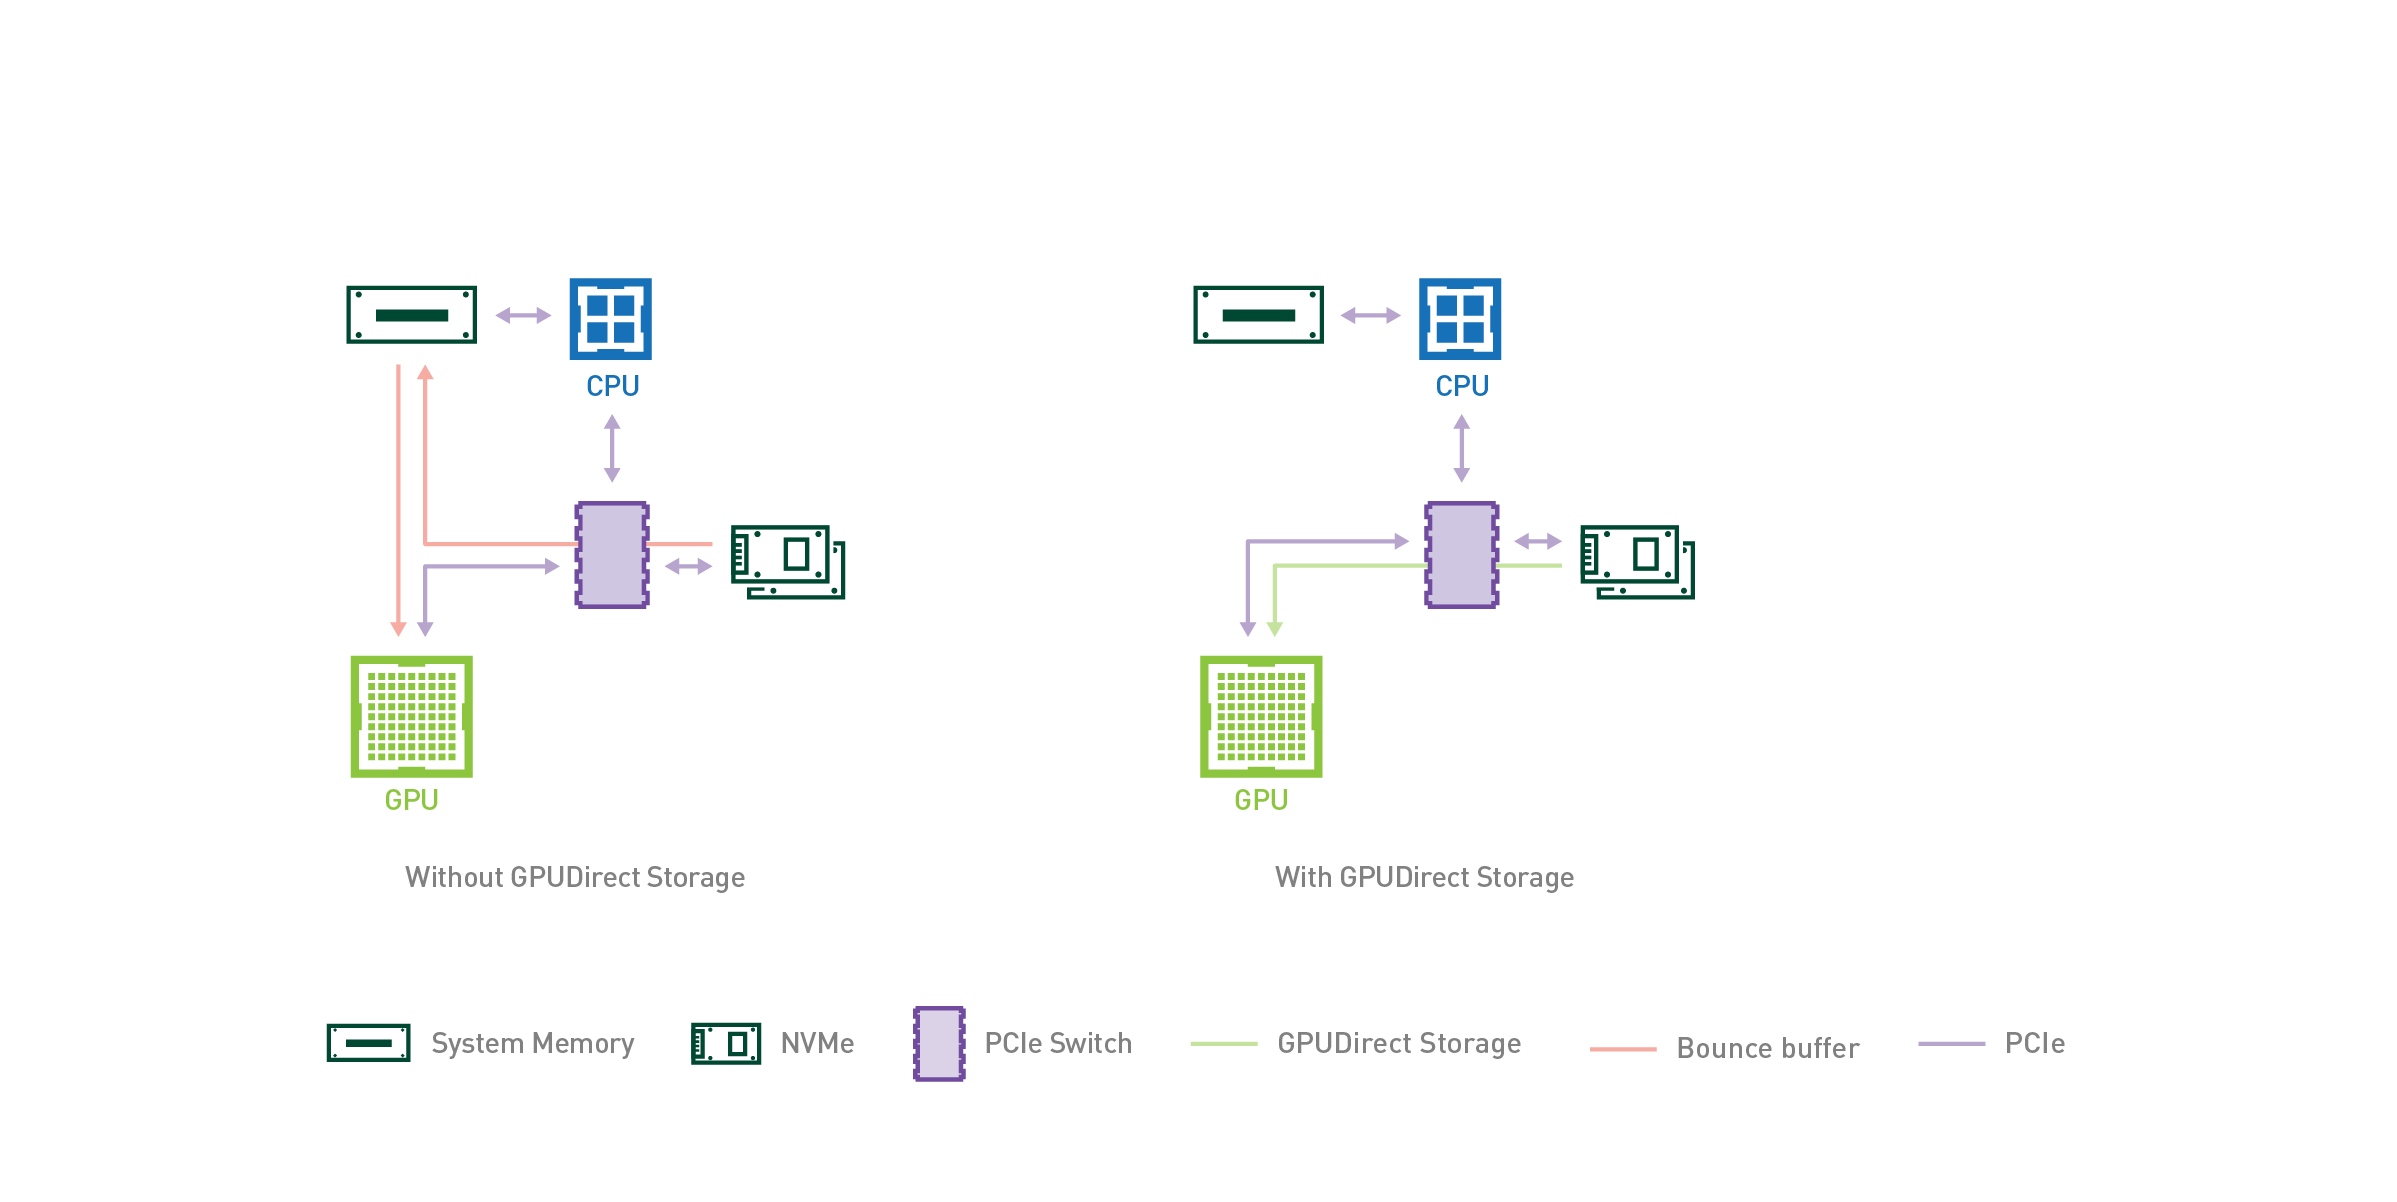
\includegraphics[scale=0.4]{GPUDirect.png}




\end{document}